%!TEX TS-program = pdflatex
%!TEX encoding = MacOSRoman

% Modello di presentazione di tesi al computer.
% Collaudato sia con LaTeX che con pdfLaTeX.
% Richide alcuni file di stile
% (marslide.sty marsdefs.sty mars-cds.sty hugefonts.sty)
% e alcune figure, che sono forniti insieme
% con questo file.
% Scritto da Gianluca Gorni
% Versione: 9 novembre 2006

\documentclass[12pt,italian,oneside]{report}

\usepackage{ifpdf}
\usepackage[italian]{babel}
\usepackage{uniudpres}
\usepackage[latin1]{inputenc}
\usepackage{pdfpages}
\usepackage{paralist}
\usepackage{bm}
\usepackage{mathrsfs}

\graphicspath{{./figure/}}

\newcounter{cap}
\setcounter{cap}{2}
\newtheorem{definiz}{Definizione}[cap]
\newtheorem{defin}[definiz]{Definizione}
\newtheorem{teor}[definiz]{Teorema}
\newtheorem{teo}{Teorema}

%% Da usare con pdfLaTeX
%% per l'eventuale conversione automatica
%% delle figure da eps in pdf:
% \usepackage{epstopdf} 
\hyperbaseurl{http://www.dimi.uniud.it/gorni/TeX/itTeXdoc/}

%% Impostazioni del documento pdf (non essenziali,
%% ma non guastano):
\hypersetup{
  % bookmarksopenlevel=2, % default
  % pdfpagelayout=SinglePage, % default
  % pdfpagemode=FullScreen, % default
  pdftitle={Progettazione e sviluppo di un'applicazione mobile cross platform per il monitoraggio di dati nautici},
  pdfauthor={Federico Zanardo},
  pdfsubject={},
  pdfkeywords={}}
  % queste informazioni su titolo-autore-soggetto-parole chiave non vengono stampate, ma sono conservate nel documento pdf (premere command-D per vederle sotto AdobeReader/AcrobatReader). Tornano buone a scopi archivistici.

% Comandi per i colori:
\newcommand{\nero}[1]{\textcolor{black}{#1}}
\newcommand{\rosso}[1]{\textcolor{red}{#1}}
\newcommand{\verdescuro}[1]{\textcolor{darkgreen}{#1}}
\newcommand{\blu}[1]{\textcolor{blue}{#1}}
\definecolor{ocra}{rgb}{.45,.24,.1}
\newcommand{\ocra}[1]{\textcolor{ocra}{#1}}
\newcommand{\sfondogiallo}[1]{\colorbox{yellow}{#1}}
\newcommand{\displaysfondogiallo}[1]{\begin{center}%
  \sfondogiallo{$\displaystyle{#1}$}\end{center}}

% Informazioni per l'intestazione
\laureando{Federico Zanardo}
\relatore[Prof.]{Ivan Scagnetto}
%\corsodilaurea{Matematica} % vecchio ordinamento
 \corsodilaureatriennale{Informatica}
% \corsodilaureaspecialistica{Fisica Computazionale}
\titolo{\huge Progettazione e sviluppo di\\ \huge un'applicazione mobile cross\\ \huge platform per il monitoraggio\\ \huge di dati nautici}
\data{16 Luglio 2020}
%\dedica{A chi mi pare}
\correlatore[Prof.]{Francesco Trevisan}
%\ignorapause
%%%%%%%%%%%%%%%%%%%%%%%%%%%%%%%%%%%%%%%%%%%%%%%%%%%%%%%
\begin{document}

\maketitle

\raggedright

%\tableofcontents
% Provare come viene l'indice a doppia colonna:
% \indicedoppiacolonna

%\chapter{Progettazione e sviluppo\label{intestazioneCapitolo}}

%%%%%%%%%%%%%%%%%%%%%%%%%%%%%%%%%%%%%%%%%

\section{Introduzione}

\begin{firstheadlineitemize}

\item \rosso{Contesto} di applicazione del progetto.

\item Hardware e software utilizzato (Raspberry, ricevitore GPS e \textit{Argos}).

\item \rosso{Classificazione} delle app mobili

\item Dart e Flutter

\begin{center}
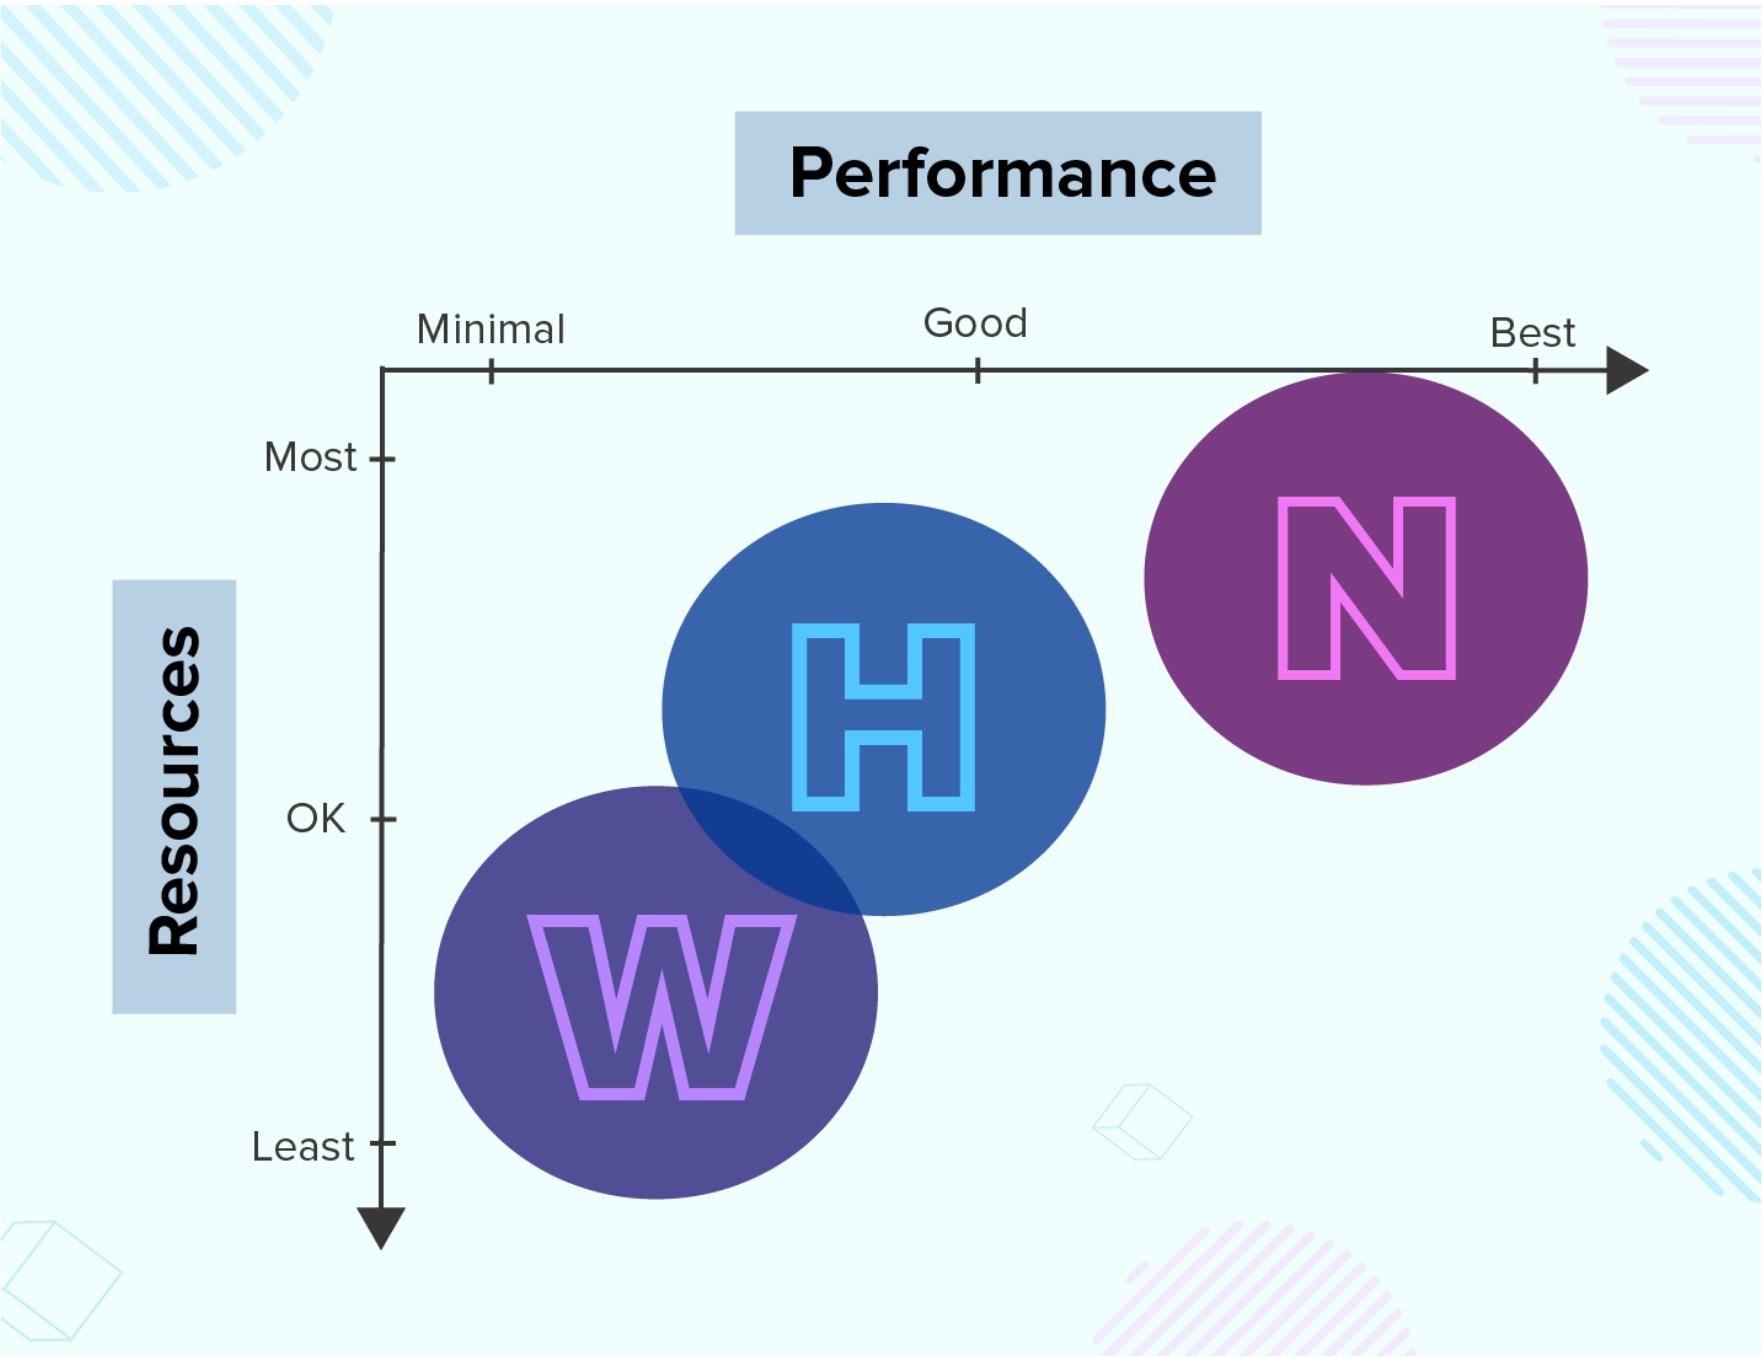
\includegraphics[scale=0.4]{native_hybrid_web}
\end{center}

\end{firstheadlineitemize}

\newpage

\section{Progettazione}

\begin{firstheadlineitemize}

\item Requisiti per l'architettura

\begin{secondheadlineitemize}

\item Flessibile
\item Strutturata
\item Facile da utilizzare per implementare funzionalita' future

\end{secondheadlineitemize}

\newpage

\item Architettura dell'applicazione

\begin{figure}[htp]
\centering
\hfill
\begin{minipage}[b]{.3\columnwidth}
\centering
  \begin{secondheadlineitemize}

\item Schermate
\item Provider
\item \rosso{BLoC}
\item Repository
\item Servizi

\end{secondheadlineitemize}
  %\caption{Didascalia della figura}\label{...}
\end{minipage}
%\hfill
\begin{minipage}[b]{.5\columnwidth}
  \begin{center}
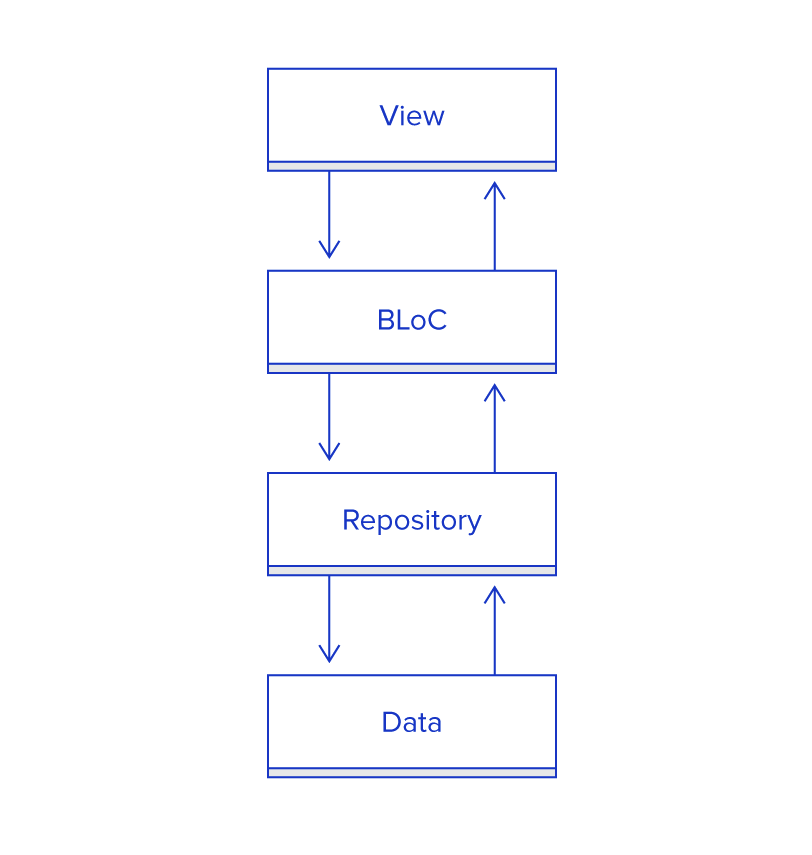
\includegraphics[scale=0.4]{architettura_implementata}
\end{center}
  %\captionof{table}{Didascalia della tabella}\label{...}
\end{minipage}\hspace*{\fill}
\end{figure}

\end{firstheadlineitemize}

\newpage

\section{Realizzazione}

\begin{firstheadlineitemize}

\item Flusso dei dati
\begin{secondheadlineitemize}
	\item Polling della socket
	\item I dati vengono salvati su una cache nel Repository
	\item I dati vengono resi disponibili ai vari BLoC dal Repository
	\item I BLoC provvedono a fornire un particolare set di dati alle schermate
	\item Le schermate visualizzano i dati ricevuti dai rispettivi BLoC
\end{secondheadlineitemize}

\newpage

\item Interfaccia grafica

\begin{figure}[htp]
\centering
\hfill
\begin{minipage}[b]{.3\columnwidth}
\centering
  \begin{secondheadlineitemize}

\item \rosso{Intuitiva}
\item Organizzata
\item Semplice

\end{secondheadlineitemize}
  %\caption{Didascalia della figura}\label{...}
\end{minipage}
%\hfill
\begin{minipage}[b]{.5\columnwidth}
%  \begin{figure}[htp]
	%\centering
	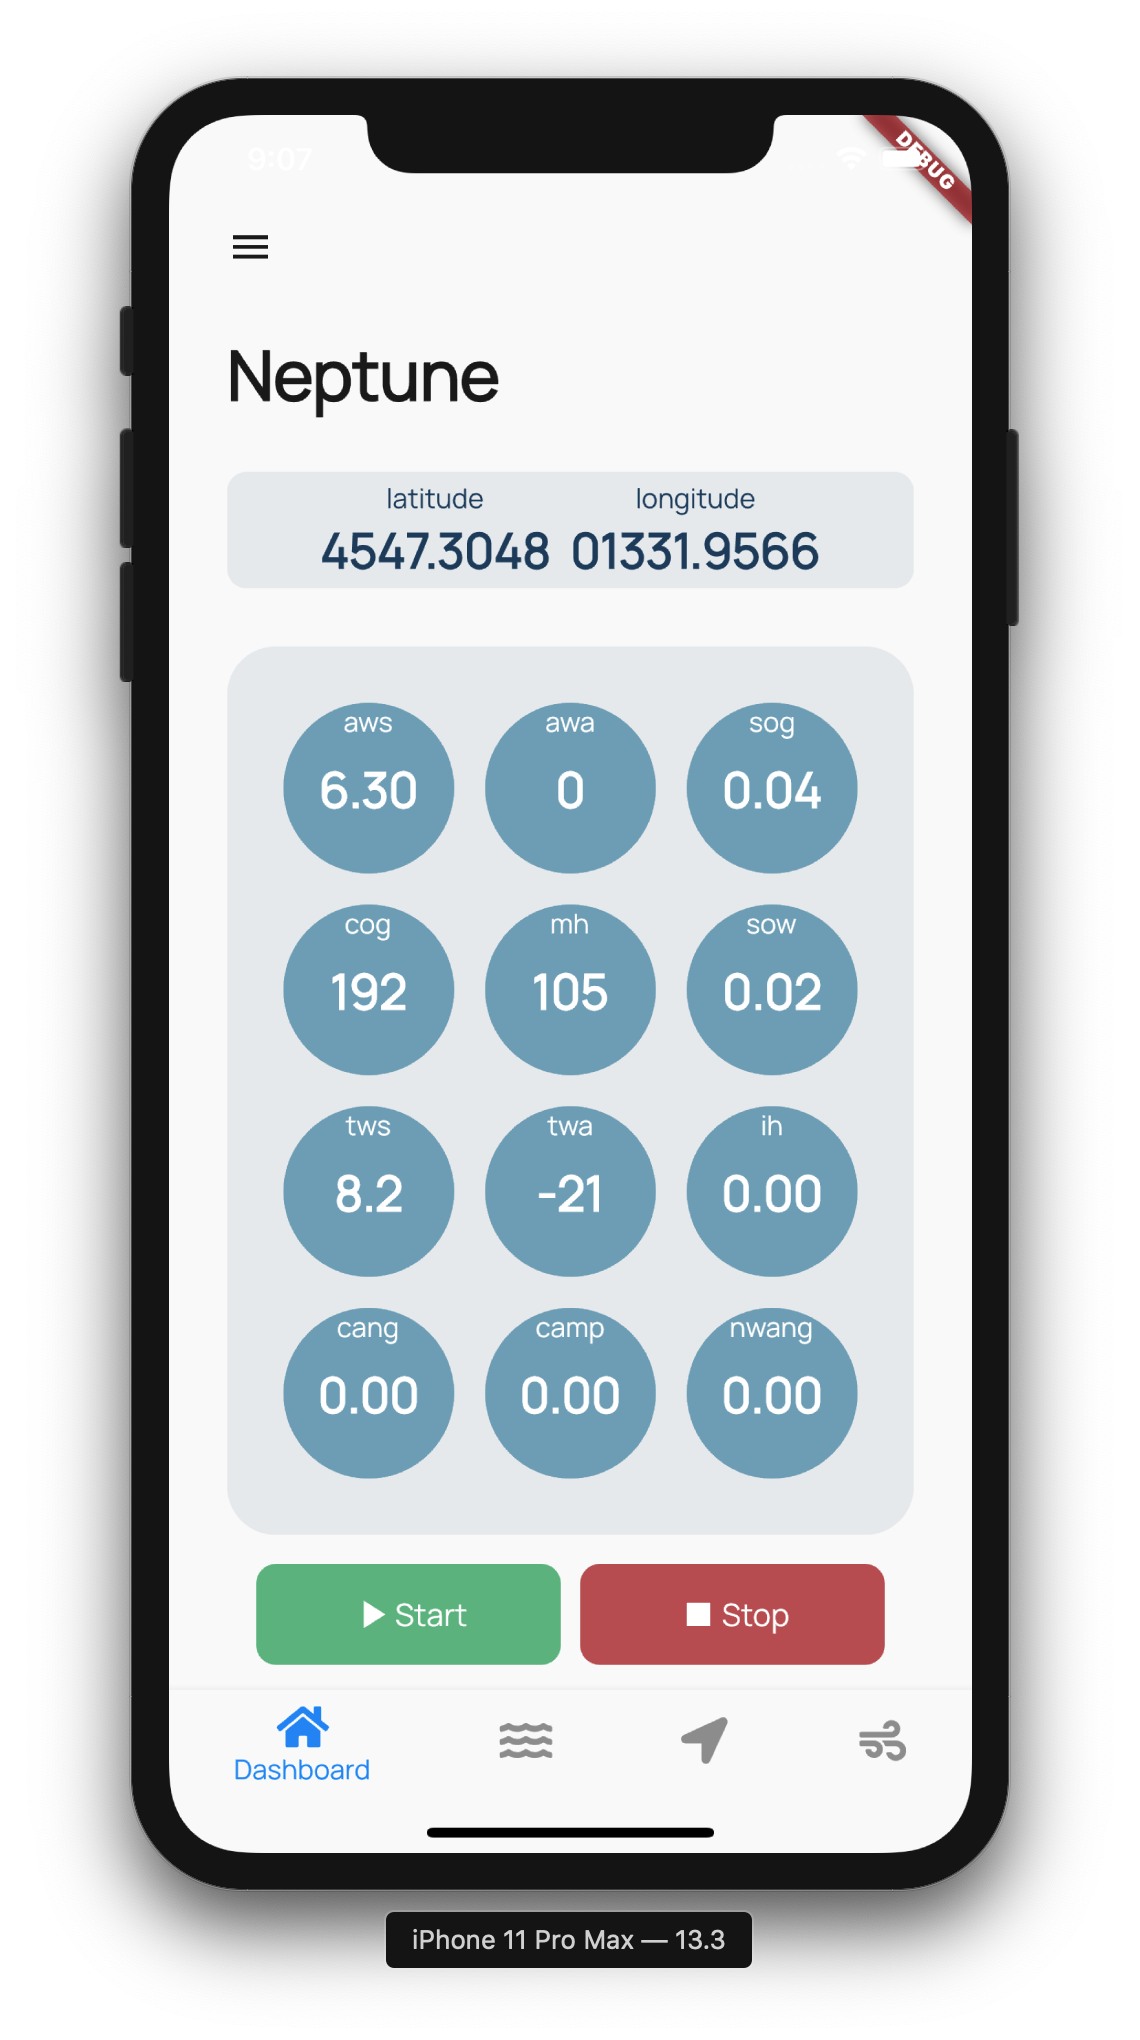
\includegraphics[scale=0.31]{dashboard}
	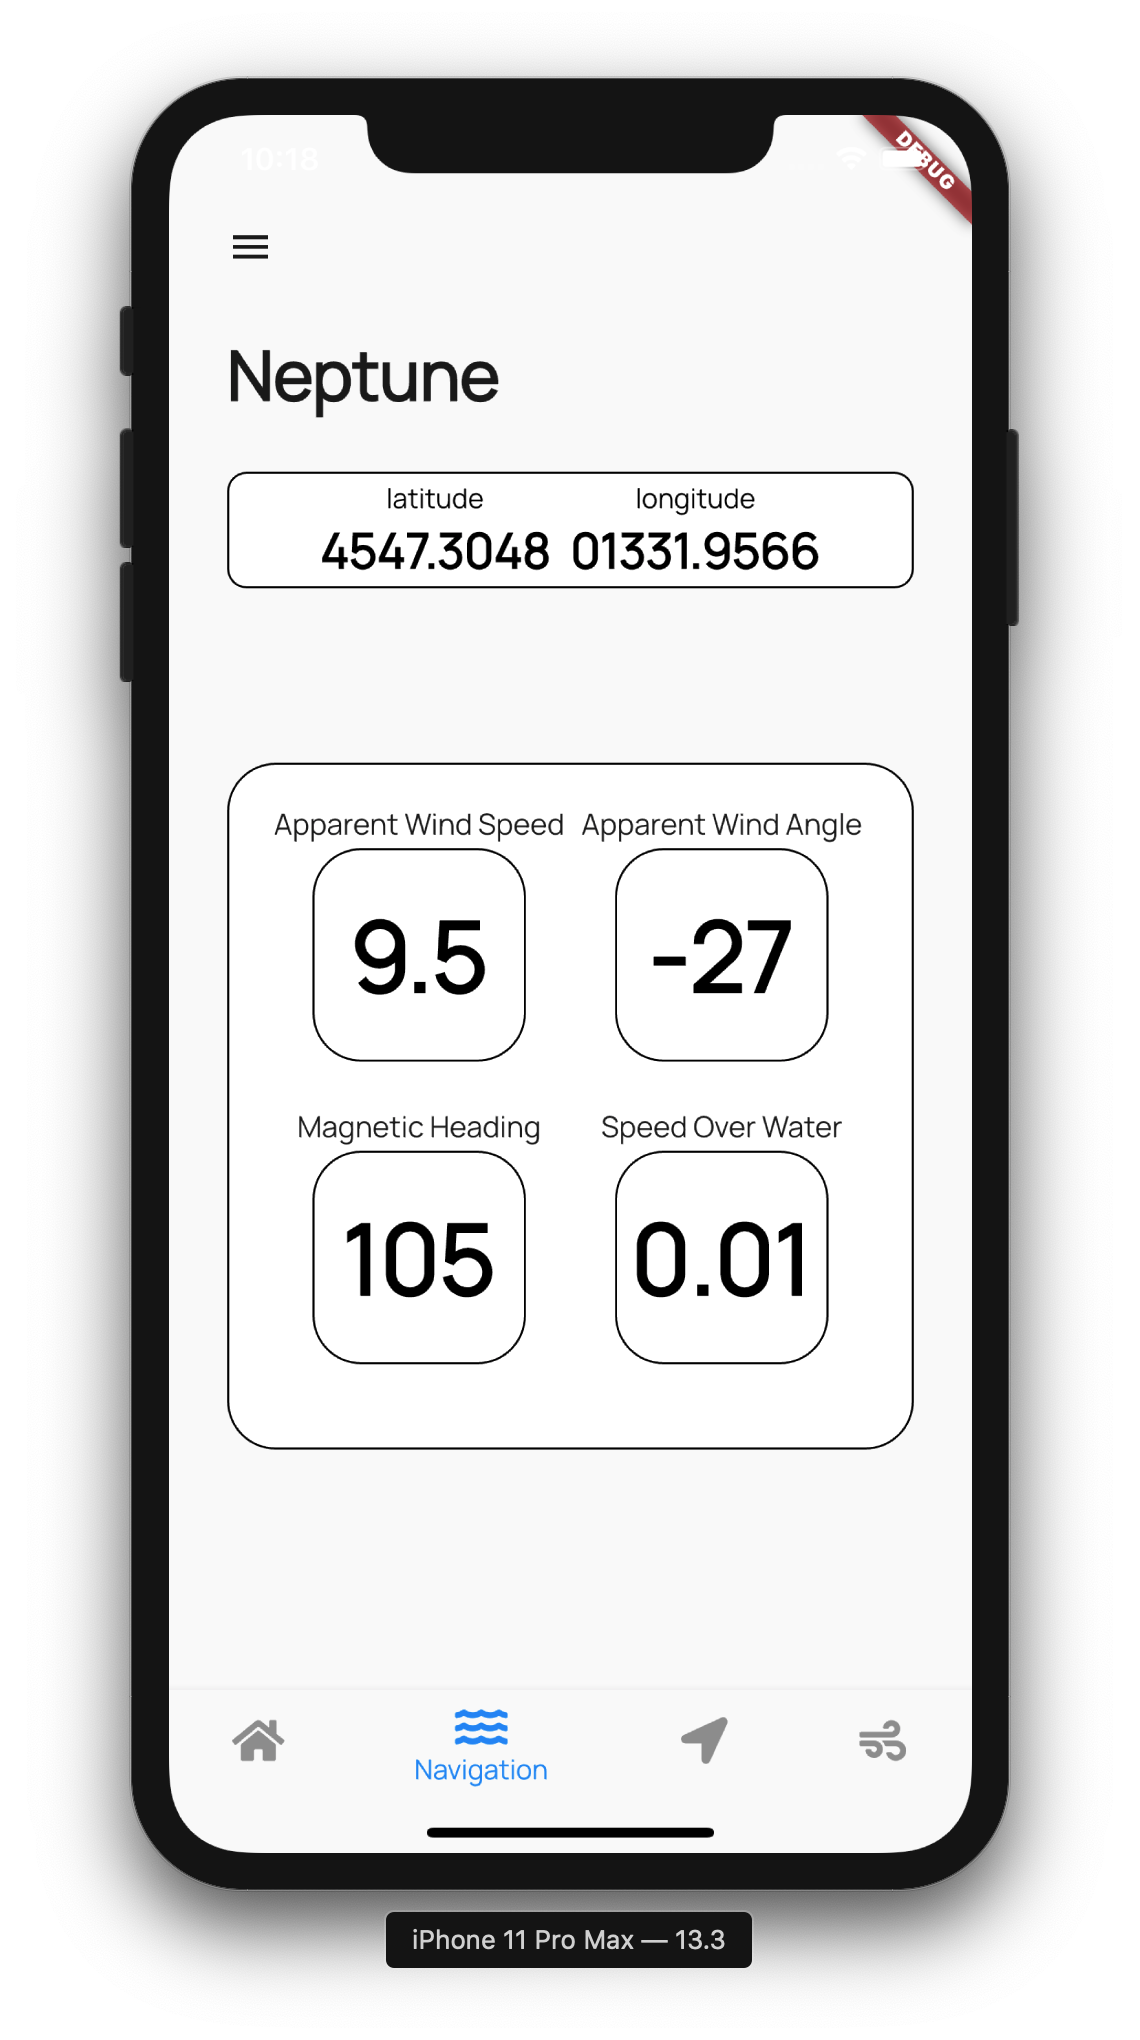
\includegraphics[scale=0.31]{navigation_high_contrast}
%\end{figure}
  %\captionof{table}{Didascalia della tabella}\label{...}
\end{minipage}\hspace*{\fill}
\end{figure}

\end{firstheadlineitemize}

%\pageTransitionBoxI

\end{document}